\begin{frame}
  \frametitle{3D Point to Pixel: Estimating the Parameters of P}
  \begin{equation*}
    \underset{\substack{\text{pixel}\\ \text{coordinate}}}{\mathbf{x}} \sim \underset{\substack{\text{trans-}\\ \text{formation}}}{\mathbf{P}}
    \underset{\substack{\text{world}\\ \text{coordinate}}}{\mathbf{X}}
  \end{equation*}  
\end{frame}

\begin{frame}
  \frametitle{Estimating Camera Parameters Given the Geometry}
  \begin{itemize}
    \item known control points
  \end{itemize}
  \begin{center}
    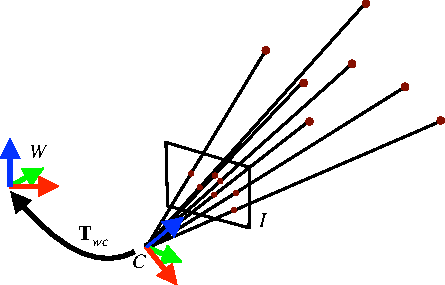
\includegraphics[width=0.5\columnwidth]{./images/dlt_3d_2d.pdf}
  \end{center}
\end{frame}

\begin{frame}
  \frametitle{Estimate Ex- and Intrinsics}
  \begin{itemize}
    \item \textbf{Wanted}: Extrinsic and intrinsic parameters of a camera
    \item \textbf{Given}: Coordinates of object points (control points)
    \item \textbf{Observed}: Coordinates of those known 3D object points in the image
  \end{itemize}
\end{frame}

\begin{frame}
  \frametitle{Mapping}
  Direct linear transform (DLT) maps any object point $\mathbf{X}$ to the image point $\mathbf{x}$.
  \begin{center}
    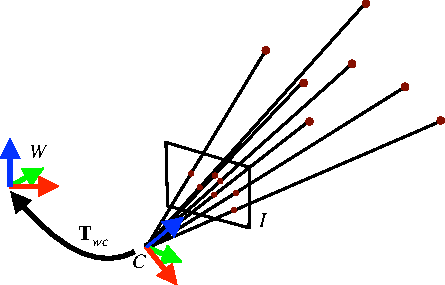
\includegraphics[width=0.5\columnwidth]{./images/dlt_3d_2d.pdf}
  \end{center}
%
  \begin{equation*}
    \vec{x} = \projectionMatrix \vec{X} \quad \text{donde} \quad
    \underset{3 \times 4}{\projectionMatrix}=\underset{3 \times 3}{\intrinsicMatrix}\underset{3 \times 4}{\begin{bmatrix} \underset{3 \times 3}{\rotation} & \underset{3 \times 1}{\translation}\end{bmatrix}}
  \end{equation*}
%
\end{frame}

% \begin{frame}
%   \frametitle{Camera Parameters}
%   \begin{itemize}
%     \item Intrinsics -- Camera-internal parameters. Given through $\intrinsicMatrix$.
%     \item Extrinsics -- Pose parameters of the camera. Given through $\rotation$ and $\vec{X}_{0}$.
%     \item Projection matrix $\projectionMatrix$ contains both, the in- and extrinsics.
%   \end{itemize}

%   \begin{align*}
%     \vec{x} &= \projectionMatrix \vec{X}\\
%     \vec{x} &= \intrinsicMatrix \begin{bmatrix} \rotation & \translation \end{bmatrix} \vec{X}\\
%     \vec{x} &= \intrinsicMatrix \rotation \begin{bmatrix} \vec{I} & -\vec{X}_{0} \end{bmatrix} \vec{X}\\
%   \end{align*}
% \end{frame}

\begin{frame}
  \frametitle{Compute the 11 intrinsic and extrinsic parameters}
  Direct Linear Transform (DLT)
  \begin{itemize}
    \item control point coordinates (given)
    \item observed image point  (given)
    \item 3 rotations, 3 translations
    \item 5 intrinsic parameters $(f_{x}, f_{y}, \principalPoint_{x}, \principalPoint_{y}, s)$
  \end{itemize}

  \begin{center}
    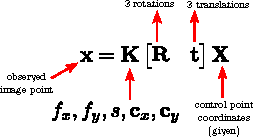
\includegraphics[width=0.5\columnwidth]{./images/projection_matrix_unknowns.pdf}
  \end{center}
\end{frame}

\begin{frame}
  \frametitle{How Many Points Are Needed?}

  \only<1-3>{
    
    Each point gives \alert{???} observation equations.

    \begin{equation*}
      \vec{x} = \projectionMatrix \vec{X}
    \end{equation*}
  }
  \only<2>{
    \begin{equation*}
      \begin{bmatrix} u\\ v\\ w\end{bmatrix} = \projectionMatrix \begin{bmatrix} U\\ V\\ W \\ T\end{bmatrix}
    \end{equation*}
  }

  \only<3>{
    \begin{equation*}
      \begin{bmatrix} \frac{u}{w}\\ \frac{v}{w}\\ 1\end{bmatrix} = \projectionMatrix \begin{bmatrix} \frac{U}{T}\\ \frac{V}{T}\\ \frac{W}{T} \\ T\end{bmatrix}
    \end{equation*}
  }

  \only<4>{
    \begin{equation*}
      \begin{bmatrix} x\\ y\\ 1\end{bmatrix} = \projectionMatrix \begin{bmatrix} X\\ Y\\ Z \\ 1\end{bmatrix}
    \end{equation*}


    \begin{align*}
      x &= \frac{p_{11}X + p_{12}Y + p_{13}Z + p_{14}}{p_{31}X + p_{32}Y + p_{33}Z + p_{34}}\\
      y &= \frac{p_{21}X + p_{22}Y + p_{23}Z + p_{24}}{p_{31}X + p_{32}Y + p_{33}Z + p_{34}}
    \end{align*}

    Each point gives \alert{two} observation equations, one for each image coordinate.
  }
\end{frame}

\begin{frame}
  \frametitle{Spatial Resection (P3P) vs. DLT}
  \begin{itemize}
    \item Calibrated camera: 
    \begin{itemize}
      \item 6 unknowns.
      \item Need at least 3 points.
      \item Problem solved by spatial resection
    \end{itemize}
    \item Uncalibrated camera: 
    \begin{itemize}
      \item 11 unknowns.
      \item Need at least 6 points 
      \item Assuming the model of an affine camera
      \item Problem solved by DLT
    \end{itemize}.
  \end{itemize}
\end{frame}

\begin{frame}
  \frametitle{DLT: Direct Linear Transform}
  Computing the Orientation of an Uncalibrated Camera using $\ge 6$ known points.
\end{frame}

\begin{frame}
  \frametitle{DLT: Problem Specification}
  \begin{itemize}
    \item Task: Estimate the 11 elements of $\projectionMatrix$.
    \item Given: 
    \begin{itemize}
      \item 3D coordinates $\mathbf{X}_{i}$ of object points.
      \item Observed image coordinates $\mathbf{x}_{i}$ of an uncalibrated camera with the mapping.
      \begin{equation*}
        \vec{x}_{i} = \projectionMatrix \vec{X}_{i} \quad i=1,\ldots,n \quad n \ge 6
      \end{equation*}
    \end{itemize}
    \item Data association
  \end{itemize}

\end{frame}

\begin{frame}
  \frametitle{Rearrange the DLT Equation}
  
  \only<1>{
    \begin{equation*}
      \vec{x}_{i} = \underset{3\times4}{\projectionMatrix} \vec{X}_{i} =
      \begin{bmatrix}
        p_{11} & p_{12} & p_{13} & p_{14} \\
        p_{21} & p_{22} & p_{23} & p_{24} \\
        p_{31} & p_{32} & p_{33} & p_{34}
      \end{bmatrix} \vec{X}_{i}
    \end{equation*}
  }

  \only<2->{
    \begin{equation*}
      \vec{x}_{i} = \underset{3\times4}{\projectionMatrix} \vec{X}_{i} =
      \begin{bNiceMatrix}[margin] 
        p_{11} & p_{12} & p_{13} & p_{14} \\
        p_{21} & p_{22} & p_{23} & p_{24} \\
        p_{31} & p_{32} & p_{33} & p_{34}
      \CodeAfter
        \tikz \node [draw=red, rounded corners, fit = (1-1) (1-last)] { } ;
        \tikz \node [draw=blue, rounded corners, fit = (2-1) (2-last)] { } ;
        \tikz \node [draw, rounded corners, fit = (3-1) (3-last)] { } ; 
      \end{bNiceMatrix} \vec{X}_{i}
    \end{equation*} 
  }
  \only<3>{
    Define the three vectors A, B and C as follows

    \begin{equation*}
      {\color{red} \boxed{\color{black}{\vec{A}}}} = \begin{bmatrix} p_{11}\\ p_{12}\\ p_{13}\\ p_{14} \end{bmatrix}, \quad
      {\color{blue} \boxed{\color{black}{\vec{B}}}} = \begin{bmatrix} p_{21}\\ p_{22}\\ p_{23}\\ p_{24} \end{bmatrix}, \quad
      \boxed{\vec{C}} = \begin{bmatrix} p_{31}\\ p_{32}\\ p_{33}\\ p_{34} \end{bmatrix}
    \end{equation*}
  }

  \only<4>{
    So what we can rewrite the equation as

    \begin{equation*}
      \vec{x}_{i} = \projectionMatrix \vec{X}_{i} =
      \begin{bNiceMatrix}[margin] 
        \vec{A}^{\top} \\
        \vec{B}^{\top} \\
        \vec{C}^{\top}
      \CodeAfter
        \tikz \node [draw=red, rounded corners, fit = (1-1) (1-last)] { } ;
        \tikz \node [draw=blue, rounded corners, fit = (2-1) (2-last)] { } ;
        \tikz \node [draw, rounded corners, fit = (3-1) (3-last)] { } ; 
      \end{bNiceMatrix} \vec{X}_{i}
    \end{equation*}
  }

  \only<5>{
    So what we can rewrite the equation as

    \begin{equation*}
      \begin{bmatrix}
        u_{i} \\
        v_{i} \\
        w_{i}
      \end{bmatrix} = 
      \vec{x}_{i} = \projectionMatrix \vec{X}_{i} =
      \begin{bNiceMatrix}[margin] 
        \vec{A}^{\top} \\
        \vec{B}^{\top} \\
        \vec{C}^{\top}
      \CodeAfter
        \tikz \node [draw=red, rounded corners, fit = (1-1) (1-last)] { } ;
        \tikz \node [draw=blue, rounded corners, fit = (2-1) (2-last)] { } ;
        \tikz \node [draw, rounded corners, fit = (3-1) (3-last)] { } ; 
      \end{bNiceMatrix} \vec{X}_{i} = 
      \begin{bmatrix}
        \vec{A}^{\top}\vec{X}_{i} \\
        \vec{B}^{\top}\vec{X}_{i} \\
        \vec{C}^{\top}\vec{X}_{i}
      \end{bmatrix}
    \end{equation*}
  }

\end{frame}

\begin{frame}
  \frametitle{Rearrange the DLT Equation}

  \begin{equation*}
    \vec{x}_{i} =
    \begin{bmatrix}
      x_{i} \\
      y_{i} \\
      1
    \end{bmatrix} =
    \begin{bmatrix}
      u_{i} \\
      v_{i} \\
      w_{i}
    \end{bmatrix} = 
    \begin{bmatrix}
      \vec{A}^{\top}\vec{X}_{i} \\
      \vec{B}^{\top}\vec{X}_{i} \\
      \vec{C}^{\top}\vec{X}_{i}
    \end{bmatrix}
  \end{equation*}

Implica

  \begin{equation*}
    x_{i} = \dfrac{u_{i}}{w_{i}} = \dfrac{\vec{A}^{\top}\vec{X}_{i}}{\vec{C}^{\top}\vec{X}_{i}}
    \quad \quad
    y_{i} = \dfrac{v_{i}}{w_{i}} = \dfrac{\vec{B}^{\top}\vec{X}_{i}}{\vec{C}^{\top}\vec{X}_{i}}
  \end{equation*}

\end{frame}

\begin{frame}
  \frametitle{Rearrange the DLT Equation}

  \begin{align*}
    x_{i} &= \dfrac{\vec{A}^{\top}\vec{X}_{i}}{\vec{C}^{\top}\vec{X}_{i}} \implies x_{i} \vec{C}^{\top}\vec{X}_{i} - \vec{A}^{\top}\vec{X}_{i} = 0\\
    y_{i} &= \dfrac{\vec{B}^{\top}\vec{X}_{i}}{\vec{C}^{\top}\vec{X}_{i}} \implies y_{i} \vec{C}^{\top}\vec{X}_{i} - \vec{B}^{\top}\vec{X}_{i} = 0
  \end{align*}

  Leads to a system of equation, which is linear in the parameters A, B and C

  \begin{align*}
    -\vec{X}_{i}^{\top}\vec{A}& &+x_{i}\vec{X}_{i}^{\top}\vec{C} &= 0 \\
    &-\vec{X}_{i}^{\top}\vec{B} &+y_{i}\vec{X}_{i}^{\top}\vec{C} &= 0
  \end{align*}

\end{frame}

\begin{frame}
  \frametitle{Estimating the Elements of $\projectionMatrix$}
  \begin{itemize}
    \item Collect elements of $\projectionMatrix$ into a parameter vector $\vec{p}$.
  \end{itemize}

  \begin{center}
    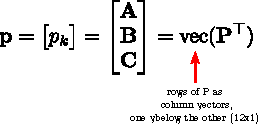
\includegraphics[width=0.5\columnwidth]{./images/projection_matrix_column_vector.pdf}
  \end{center}
  
\end{frame}

\begin{frame}
  \frametitle{Solving the Linear System (Homogeneous System => SVD)}
  \begin{itemize}
    \item Solve $A\mathbf{p}=0$ via SVD.
    \item Choose $\mathbf{p}$ as singular vector of smallest singular value.
  \end{itemize}
  % \includegraphics[width=0.6\textwidth]{placeholder-image.jpg}
\end{frame}

\begin{frame}
  \frametitle{Redundant Observations}
  \begin{itemize}
    \item Minimize $\|A\mathbf{p}\|$ with $\|\mathbf{p}\|=1$.
    \item Use SVD to find best solution.
  \end{itemize}
  % \includegraphics[width=0.7\textwidth]{placeholder-image.jpg}
\end{frame}

\begin{frame}
  \frametitle{Critical Surfaces}
  \begin{itemize}
    \item $M$ is of rank 11 if number of points $\ge 6$.
    \item No solution if all points lie on a plane.
  \end{itemize}
  % \includegraphics[width=0.65\textwidth]{placeholder-image.jpg}
\end{frame}

\begin{frame}
  \frametitle{From $P$ to $K,R,t$}
  % \includegraphics[width=0.6\textwidth]{placeholder-image.jpg}
\end{frame}

\begin{frame}
  \frametitle{Decomposition of P}
  \begin{itemize}
    \item Compute $K, R, t$ from $P$.
    \item Use QR decomposition for rotation and calibration matrices.
  \end{itemize}
  % \includegraphics[width=0.7\textwidth]{placeholder-image.jpg}
\end{frame}

\begin{frame}
  \frametitle{DLT in a Nutshell}
  \begin{enumerate}
    \item Build matrix $M$ for linear system $M p = 0$.
    \item Solve by SVD.
    \item Decompose $P$ to obtain $K,R,t$.
  \end{enumerate}
  % \includegraphics[width=0.6\textwidth]{placeholder-image.jpg}
\end{frame}

\begin{frame}
  \frametitle{Discussion DLT}
  \begin{itemize}
    \item Solution unstable if control points nearly planar.
    \item Not statistically optimal.
  \end{itemize}
  % \includegraphics[width=0.7\textwidth]{placeholder-image.jpg}
\end{frame}

\begin{frame}
  \frametitle{Summary}
  \begin{itemize}
    \item Direct linear transform estimates intrinsic and extrinsic camera parameters.
    \item Needs at least 6 control points.
    \item Provides direct solution.
  \end{itemize}
  % \includegraphics[width=0.7\textwidth]{placeholder-image.jpg}
\end{frame}

\begin{frame}
  \frametitle{Literature}
  \begin{itemize}
    \item Förstner \& Wrobel, Photogrammetric Computer Vision, Chapter 11.2
    \item Förstner, Scriptum Photogrammetrie I, Chapter 13.3
  \end{itemize}
  % \includegraphics[width=0.5\textwidth]{placeholder-image.jpg}
\end{frame}

\begin{frame}
  \frametitle{Slide Information}
  \begin{itemize}
    \item Slides created by Cyrill Stachniss for Photogrammetry and Robotics courses.
    \item Acknowledgements and notes in original slides.
  \end{itemize}
  % \includegraphics[width=0.5\textwidth]{placeholder-image.jpg}
\end{frame}

\begin{frame}
  \frametitle{Material: Direct Linear Transform}

  Direct Linear Transform for Camera Calibration and Localization (Cyrill Stachniss)
  \url{https://youtu.be/3NcQbZu6xt8}

  Camera Calibration using Zhang's Method (Cyrill Stachniss)
  \url{https://youtu.be/-9He7Nu3u8s}

  Intrinsic and Extrinsic Matrices | Camera Calibration
  \url{https://youtu.be/2XM2Rb2pfyQ}

\end{frame}
